\section{Proposed Method}
\label{sec:method}


\begin{figure*}[t]
    \centering
    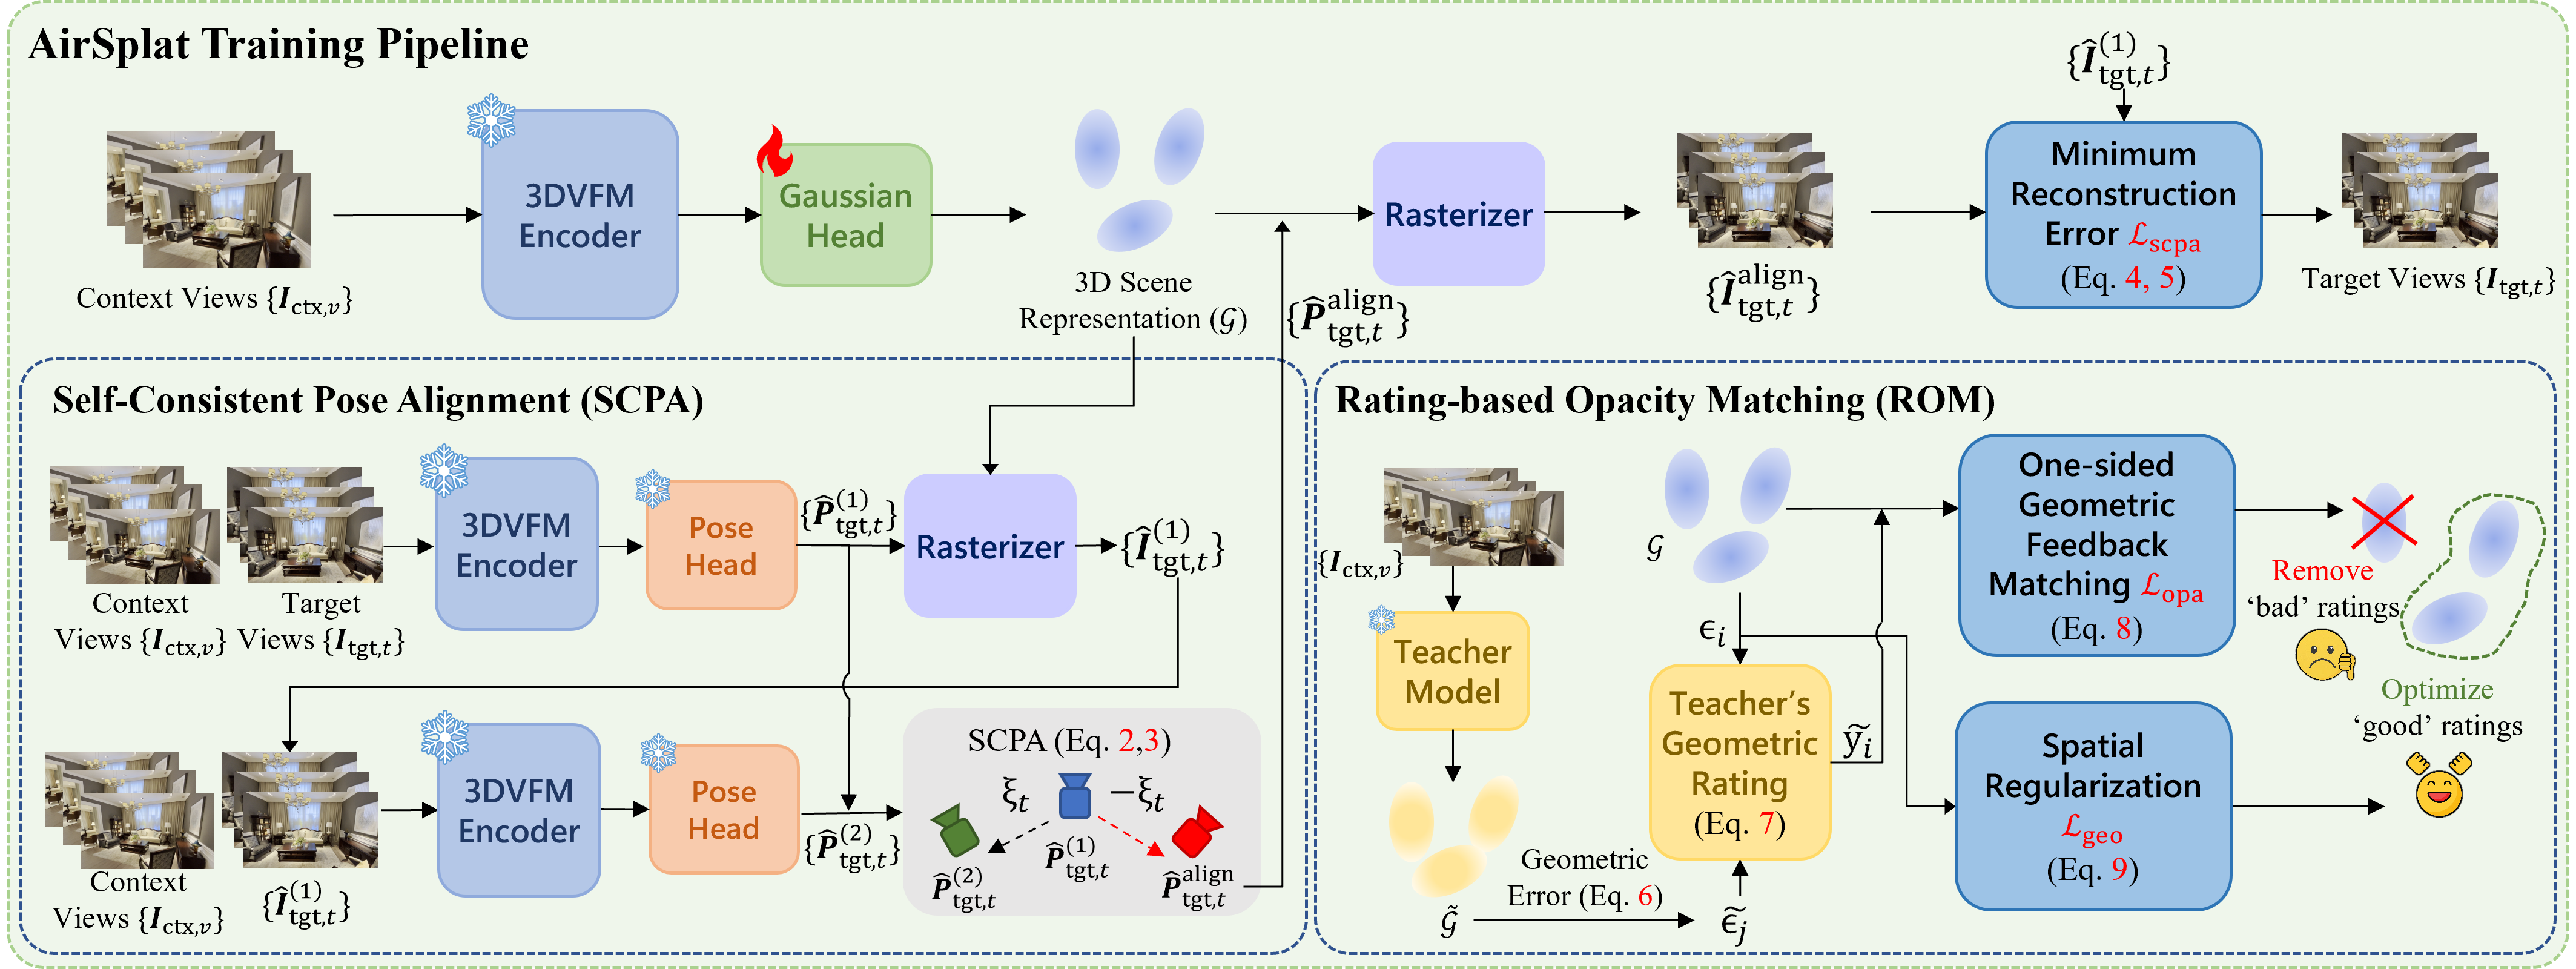
\includegraphics[width=\linewidth]{figures/main_architecture.png}
    \caption{\textbf{Overview of our AirSplat training pipeline.} During training of a Gaussian head of a 3DVFM, the encoder and its pose head are frozen. Our SCPA module corrects the predicted target pose to align the rendered target views to the GT target views. Our ROM module gathers the geometric feedback from the teacher model, and based on the feedback, it enhances the multi-view consistency of the predicted 3D primitives.}
    \label{fig:main_architecture}
    \vspace{-3mm}
\end{figure*}

\subsection{Overview of AirSplat}
Given a set of $V$ uncalibrated input context views $\mathcal{I}_\text{ctx} = \{\bm{I}_{\text{ctx},v}\}_{v=1}^V$, our model $f_{\phi}$ predicts a set of $N$ pixel-aligned 3D Gaussian primitives $\mathcal{G} = \{g_i\}_{i=1}^N$ alongside the estimated context camera intrinsics $\hat{\mathcal{K}}_\text{ctx} = \{\hat{\bm{K}}_{\text{ctx},v}\}_{v=1}^V$ and extrinsics $\hat{\mathcal{P}}_\text{ctx} = \{\hat{\bm{P}}_{\text{ctx},v}\}_{v=1}^V$. Each individual Gaussian primitive $g_i$ is explicitly parameterized by its 3D mean position $\bm{\mu}_i \in \mathbb{R}^3$, covariance matrix $\bm{\Sigma}_i$, opacity $\alpha_i \in [0, 1]$, and color $\bm{c}_i$. 
To adapt $f_{\phi}$ for high-fidelity NVS while preserving its foundational priors, we freeze the main 3DVFM encoder and geometry heads, optimizing only the Gaussian prediction head. Our overall training framework is then driven by two core modules: Self-Consistent Pose Alignment (SCPA), which dynamically resolves pose-geometry discrepancies during target view rendering, and Rating-based Opacity Matching (ROM), which systematically prunes hallucinated artifacts using geometric feedback from a teacher model.

\begin{figure*}[t]
    \centering
    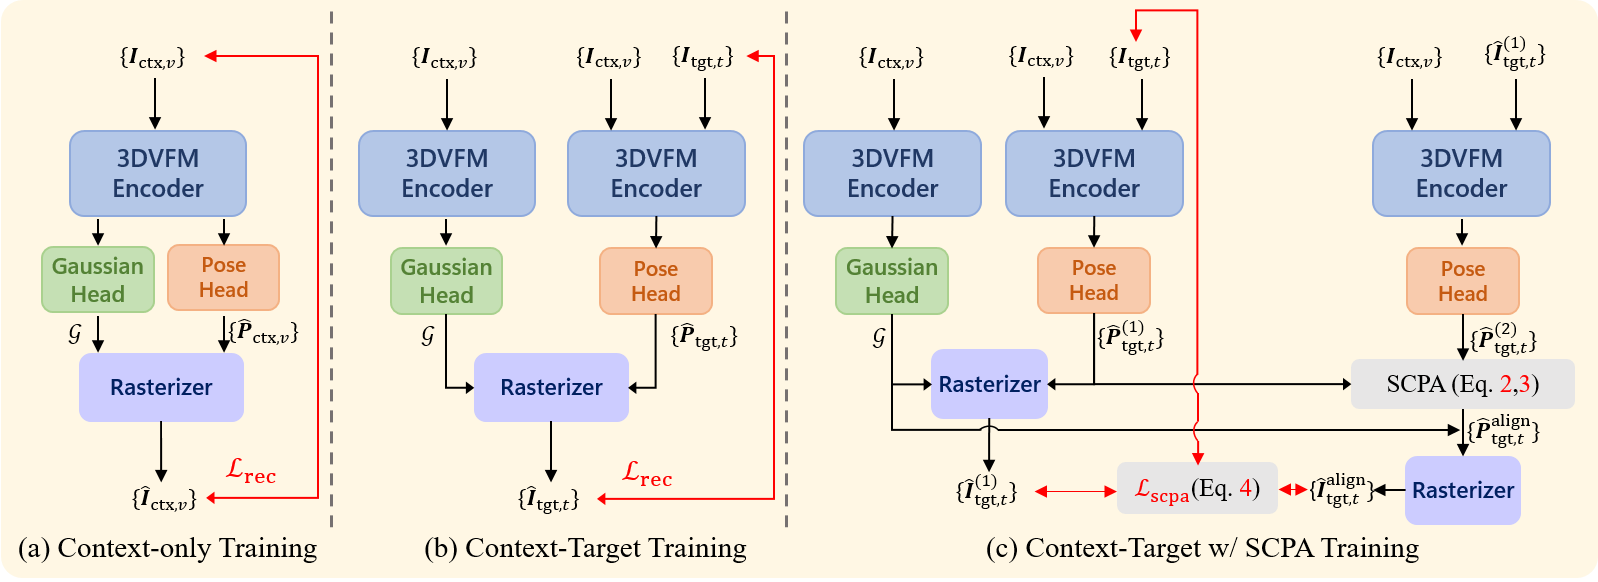
\includegraphics[width=0.9\linewidth]{figures/pose_corr.png}
    \vspace{-1mm}
    \caption{\textbf{Comparison of training paradigms in pose-free NVS.} (a) Training with the context-only strategy, adopted in \cite{jiang2025anysplat}, leads to a lack of direct supervision for novel viewpoints. (b) The context-target strategy, following \cite{huang2025no}, results in spatial misalignment. (c) Our SCPA corrects the inherent spatial drift, enabling the network to learn both structurally consistent 3D geometry and robust novel view synthesis.}
    \label{fig:pose_corr}
    \vspace{-5mm}
\end{figure*}

\subsection{Self-Consistent Pose Alignment (SCPA)}
\label{sec:scpa}

\noindent \textbf{Pose-Geometry Discrepancy.} 
During pose-free NVS training, $\mathcal{G}$ is optimized by rasterizing it onto the image-space using a set of predicted target camera parameters $(\hat{\mathcal{P}}_\text{tgt} = \{\hat{\bm{P}}_{\text{tgt},t}\}_{t=1}^T, \hat{\mathcal{K}}_\text{tgt} = \{\hat{\bm{K}}_{\text{tgt},t}\}_{t=1}^T)$ corresponding to $T$ ground-truth target views $\mathcal{I}_\text{tgt} = \{\bm{I}_{\text{tgt},t}\}_{t=1}^T$. 
This rasterization process yields the synthesized target images $\hat{\mathcal{I}}_\text{tgt} = \{\hat{\bm{I}}_{\text{tgt},t}\}_{t=1}^T$. Fig.~\ref{fig:pose_corr} illustrates two prevailing paradigms for sampling these views during training. 
The context-only approach, following \cite{jiang2025anysplat}, trivially restricts $\mathcal{I}_\text{tgt}$ to be identical to $\mathcal{I}_\text{ctx}$, leading to lack of direct supervision for novel viewpoints. Conversely, SPFSplat \cite{huang2025no} introduces a context-target strategy, sampling target views $\mathcal{I}_\text{tgt}$ that are spatially distinct from $\mathcal{I}_\text{ctx}$. This necessitates an additional forward pass to estimate $(\hat{\mathcal{P}}_\text{tgt}, \hat{\mathcal{K}}_\text{tgt})$ by feeding the concatenation of $\mathcal{I}_\text{ctx}$ and $\mathcal{I}_\text{tgt}$ into the 3DVFM.  While this disentanglement improves robustness to interpolated views since the 3D primitives $\mathcal{G}$ are derived solely from $\mathcal{I}_\text{ctx}$ and supervised by distinct target observations, it introduces a critical structural flaw. Specifically, the asymmetric information flow, where geometry extraction relies exclusively on context views while pose estimation relies on both context and target views, induces a fundamental \textit{pose-geometry discrepancy} during training. As illustrated in Fig.~\ref{fig:pose_corr_diff}, the error between the rendered view $\hat{\bm{I}}_{\text{tgt},t}$ (`Rendered View w/ $\hat{\bm{P}}_{\text{tgt},t}$') and $\bm{I}_{\text{tgt},t}$ (GT target View) is dominated by spatial misalignment rather than photometric degradation, which is the consequence of the \textit{pose-geometry discrepancy}. When supervised directly via a pixel-wise reconstruction loss, this extrinsic spatial shift yields corrupted gradients, resulting in unstable optimization.


% Instead of refining the underlying 3D structure, the optimizer compensates for the pose error by spatially dilating ("blurring") the Gaussians or introducing floating artifacts.  Consequently, the model fails to capture sharp, physically consistent scene geometry.

% \begin{figure*}[t]
%     \centering
%     \includegraphics[width=0.95\linewidth]{figures/pose_corr_diff.png}
%     \caption{\textbf{Effect of Self-Consistent Pose Alignment (SCPA).} We compare rendered target views using the initial predicted pose $\hat{\bm{P}}^{(1)}_{\text{tgt},t}$, our aligned pose $\hat{\bm{P}}_{\text{tgt},t}^\text{align}$ against the ground truth, during training. As highlighted by the red arrows, the initial pose prediction results in a noticeable spatial shift, evident in the misaligned structural lines on the ground.
%     Our proposed SCPA corrects the inherent spatial drift and ensures that the model learn structurally consistent 3D geometry and robust NVS. In the error maps, blue indicates small errors, and red indicates large errors.}
%     \label{fig:pose_corr_diff}
%     \vspace{-3mm}
% \end{figure*}

\noindent \textbf{Self-Consistent Pose Alignment.} 
To mitigate this pose-geometry discrepancy, we propose \textit{Self-Consistent Pose Alignment} (SCPA), a self-correcting strategy that mathematically quantifies and reverses the spatial drift induced by the context-target training strategy, rather than directly applying photometric supervision on misaligned renderings. 
% Rather than directly applying photometric supervision on misaligned renderings, SCPA introduces a self-correcting loop. 
Based on the predicted $\mathcal{G}$ from $\mathcal{I}_\text{ctx}$ and the initial target pose estimates $\hat{\mathcal{P}}^{(1)}_\text{tgt}$ from the concatenation of ($\mathcal{I}_\text{ctx}, \mathcal{I}_\text{tgt}$), we first render an initial set of synthesized target images $\hat{\mathcal{I}}^{(1)}_\text{tgt}$. We then feed the concatenation of $\mathcal{I}_\text{ctx}$ and $\hat{\mathcal{I}}^{(1)}_\text{tgt}$ back into $f_{\phi}$ to yield a second set of pose predictions:
\begin{equation}
    \hat{\mathcal{P}}^{(2)}_\text{tgt} = f_{\phi}(\mathcal{I}_\text{ctx}, \hat{\mathcal{I}}^{(1)}_\text{tgt}).
    \label{eq:recursive_pose}
\end{equation}
Empirically, rendering a second set of images $\hat{\mathcal{I}}^{(2)}_\text{tgt}$ from $\hat{\mathcal{P}}^{(2)}_\text{tgt}$ reveals that $f_{\phi}$ exhibits a systematic, repeated drift when mapping synthesized geometry back to the pose manifold (see \textit{Suppl.} for detailed visualizations). From this observation, we propose to compute the corrected poses $\hat{\mathcal{P}}^{\text{align}}_\text{tgt} = \{\hat{\bm{P}}^{\text{align}}_{\text{tgt},t}\}_{t=1}^T$ that better align with the predicted scene geometry space by reversing the observed pose discrepancy between $\hat{\bm{P}}^{(\text{1})}_{\text{tgt}, t}$ and $\hat{\bm{P}}^{(\text{2})}_{\text{tgt}, t}$.

\begin{figure*}[t]
    \centering
    \includegraphics[width=0.95\linewidth]{figures/pose_corr_diff.pdf}
    \caption{\textbf{Effect of Self-Consistent Pose Alignment (SCPA).} We compare rendered target views using the initial predicted pose $\hat{\bm{P}}^{(1)}_{\text{tgt},t}$, our aligned pose $\hat{\bm{P}}_{\text{tgt},t}^\text{align}$ against the ground truth, during training. As highlighted by the red arrows, the initial pose prediction results in a noticeable spatial shift, evident in the misaligned structural lines on the ground.
    Our proposed SCPA corrects the inherent spatial drift and ensures that the model learn structurally consistent 3D geometry and robust NVS. In the error maps, blue indicates small errors, and red indicates large errors.}
    \label{fig:pose_corr_diff}
    \vspace{-3mm}
\end{figure*}
To approximate the aligned pose $\hat{\bm{P}}^{\text{align}}_{\text{tgt}, t}$, we compute the relative transformation between the initial prediction $\hat{\bm{P}}^{(1)}_{\text{tgt}, t}$ and the re-predicted pose $\hat{\bm{P}}^{(2)}_{\text{tgt}, t}$. We denote  this transformation as $\bm{\xi}_t$ which is a 6-vector of coordinates in the Lie algebra $\mathfrak{se}(3)$:
\begin{equation}
    \bm{\xi}_t = \log\left(\hat{\bm{P}}^{(2)}_{\text{tgt}, t} (\hat{\bm{P}}^{(1)}_{\text{tgt}, t})^{-1}\right)^{\vee},
\end{equation}
where $\log(\cdot)^{\vee}: \text{\textbf{SE}(3)} \to \mathfrak{se}(3)$ denotes the logarithm map \cite{DBLP:journals/corr/abs-2103-15980}. To perform the self-consistent pose alignment, we back-extrapolate along the manifold by negating $\bm{\xi}_t$. This negated vector is mapped back to the $\text{\textbf{SE}(3)}$ manifold via the exponential map $\exp(\cdot^{\wedge}): \mathfrak{se}(3) \to \text{\textbf{SE}(3)}$ and applied to $\hat{\bm{P}}^{(1)}_{\text{tgt}, t}$:
\begin{equation}
    \hat{\bm{P}}_{\text{tgt},t}^{\text{align}} = \exp\left((-\bm{\xi}_t)^{\wedge}\right) \hat{\bm{P}}^{(1)}_{\text{tgt}, t}.
\end{equation}
Finally, to ensure training stability and prevent degradation in cases where the re-prediction fails, we employ a minimum-error supervision strategy. We render the aligned images $\hat{\mathcal{I}}^{\text{align}}_\text{tgt}$ from $\hat{\mathcal{P}}^\text{align}_\text{tgt}$, and define the $\mathcal{L}_{\text{scpa}}$ as the minimum reconstruction error between the aligned $\hat{\bm{I}}^{\text{align}}_{\text{tgt},t}$ and initial $\hat{\bm{I}}^{(1)}_{\text{tgt},t}$ renderings:
\begin{equation}
    \mathcal{L}_{\text{scpa}} = \sum_{t=1}^{T} \min\left(\mathcal{L}_{\text{rec}}(\hat{\bm{I}}^{\text{align}}_{\text{tgt},t}, \bm{I}_{\text{tgt},t}), \mathcal{L}_{\text{rec}}(\hat{\bm{I}}^{(1)}_{\text{tgt},t}, \bm{I}_{\text{tgt},t}) \right).
\end{equation}
Following standard practices~\cite{xu2025depthsplat, chen2024mvsplat}, $\mathcal{L}_{\text{rec}}$ is defined as a weighted sum of the Mean Squared Error (MSE) and the LPIPS perceptual metric \cite{zhang2018perceptual}:
\begin{equation}
    \mathcal{L}_{\text{rec}}(\hat{\bm{I}}_{\text{tgt}}, \bm{I}_{\text{tgt}}) =  \| \hat{\bm{I}}_{\text{tgt}} - \bm{I}_{\text{tgt}} \|_2^2 + \lambda_{s} \text{LPIPS}(\hat{\bm{I}}_{\text{tgt}}, \bm{I}_{\text{tgt}}).
\end{equation}
By dynamically supervising the model with the aligned viewpoint, SCPA effectively suppresses the emergence of artifacts caused by the pose-geometry discrepancy of the context-target training strategy.


% \subsection{Self-Consistent Pose Alignment (SCPA)}

% \noindent \textbf{Pose-geometry Discrepancy in Pose-free NVS Training.} 
% During pose-free NVS training, the 3D representation $\mathcal{G}$ are rasterized onto the predicted target cameras information ($\hat{\mathcal{P}}_\text{tgt} = \{\hat{\bm{P}}_{\text{tgt},t}\}_{t=1}^T$, $\hat{\mathcal{K}}_\text{tgt} = \{\hat{\bm{K}}_{\text{tgt},t}\}_{t=1}^T$) corresponding to $T$ ground-truth target views $\mathcal{I}_\text{tgt} = \{\bm{I}_{\text{tgt},t}\}_{t=1}^T$. The rasterization process generates $T$ synthesized target images $\hat{\mathcal{I}}_\text{tgt} = \{\hat{\bm{I}}_{\text{tgt},t}\}_{t=1}^T$. Fig.~\ref{fig:pose_corr} shows two common designs for sampling target views. The context-only approach \cite{jiang2025anysplat} simply sets the target views $\mathcal{I}_\text{tgt}$ as the context views $\mathcal{I}_\text{ctx}$. SPFSplat \cite{huang2025no} propose the context-target strategy which samples novel $\mathcal{I}_\text{tgt}$ different from $\mathcal{I}_\text{ctx}$. This approach adopts one more foward-pass to compute the target cameras information ($\hat{\mathcal{P}}_\text{tgt}$, $\hat{\mathcal{K}}_\text{tgt}$) by feeding the concatenation of $\mathcal{I}_\text{ctx}$ and $\mathcal{I}_\text{tgt}$ to $f_{\phi}$. As the 3D primitives $\mathcal{G}$ are solely estimated from $\mathcal{I}_\text{ctx}$, this strategy enhances the model's robutsness towards interpolated views. However, the asymmetric information flow of predicting $\mathcal{G}$ and ($\hat{\mathcal{P}}_\text{tgt}$, $\hat{\mathcal{K}}_\text{tgt}$) creates a fundamental \textit{pose-geometry discrepancy} during training. Our Fig.~\ref{fig:pose_corr_diff} illustrates this phenomenom by showcasing an example of a pair of $\hat{\bm{I}}_{\text{tgt},t}$ (`Rendered View w/ $\hat{\bm{P}}_{\text{tgt},t}$') and $\bm{I}_{\text{tgt},t}$ (GT target View) and their error map. We can observe that the large discrepancy between the two images are mainly due the misalignment not the rendering quality. When supervised by the  reconstruction loss, this misalignment propagates suboptimal gradients. Instead of refining the true 3D structure, the optimizer is forced to "blur" the Gaussians or introduce floating artifacts to compensate for the spatial shift caused by the pose error. Consequently, the model fails to capture sharp, consistent scene geometry, leading to degraded synthesis quality.

% \begin{figure*}[t]
%     \centering
%     \includegraphics[width=\linewidth]{figures/pose_corr_diff.png}
%     \caption{Effect of our Self-Consistent Pose Alignment. Rendered target views using $\hat{\bm{P}}_{\text{tgt}}$ and $\hat{\bm{P}}_{\text{tgt}}^\text{align}$ and ground truth.}
%     \label{fig:pose_corr_diff}
% \end{figure*}


% \noindent \textbf{Self-Consistent Pose Alignment.} 
%  We propose the \textit{Self-Consistent Pose Alignment} (SCPA), a training-time refinement mechanism that leverages the robust relative pose estimation capability of 3DVFMs. Instead of directly supervising our model with the misaligned renderings, we introduce a self-correcting feedback loop. 
% Given the predicted Gaussians $\mathcal{G}$ and the initial predicted target poses $\hat{\mathcal{P}}^1_\text{tgt}$, we render the first synthesized target images set $\hat{\mathcal{I}}^1_\text{tgt}$.
% We feed the concatenation of $\mathcal{I}_\text{ctx}$ and $\hat{\mathcal{I}}^1_\text{tgt}$ again to $f_{\phi}$ to predict the second predicted target poses $\hat{\mathcal{P}}^2_\text{tgt}$:
% \begin{equation}
%     \hat{\mathcal{P}}^2_\text{tgt} = f_{\phi}(\mathcal{I}_\text{ctx}, \hat{\mathcal{I}}^1_\text{tgt}).
% \end{equation}
% By rendering another $\hat{\mathcal{I}}^2_\text{tgt}$ from $\mathcal{G}$ and $\hat{\mathcal{P}}^2_\text{tgt}$ and comparing $\hat{\mathcal{I}}^1_\text{tgt}, \hat{\mathcal{I}}^2_\text{tgt}, \mathcal{I}_\text{tgt}$, we observe an interesting phenomenom that $f_{\phi}$ produces a repeated tendency of misalignemt (Fig.XX and more visualizations in \textit{Suppl.}). From this observation, we propose to instant compute the $\hat{\mathcal{P}}^{\text{align}}_\text{tgt}$ having better alignemnt with  $\mathcal{I}_\text{tgt}$ by reversing the discrepancy of $\hat{\mathcal{P}}^1_\text{tgt}$ and $\hat{\mathcal{P}}^2_\text{tgt}$. Please note that $\hat{\mathcal{I}}^2_\text{tgt}$ rendering is only conducted when we explore the problem, in the final training strategy we only need $\hat{\mathcal{P}}^2_\text{tgt}$.


% To align the rendering coordinate system with the target observation, we perform a first-order bias correction in the Lie algebra SE(3) \cite{}. By back-extrapolating the estimated bias, we derive the final aligned pose $\hat{\bm{P}}_{\text{tgt}, t}^\text{align}$:
% \begin{equation}
%     \hat{\bm{P}}_{\text{tgt}, t}^\text{align} = \hat{\mathbf{P}}_{\text{tgt}, t}^{2} \cdot (\hat{\mathbf{P}}_{\text{tgt}, t})^{-1} \cdot \hat{\bm{P}}_{\text{tgt}, t},
% \end{equation}
% where $\log(\cdot)$ and $\exp(\cdot)$ denote the logarithm and exponential maps for $SE(3)$, respectively. From $\hat{\bm{P}}_{\text{tgt}, t}^\text{align}$ we render $\hat{\mathcal{I}}^{\text{align}}_\text{tgt}$.

% Finally, our reconstruction optimization is the mean of mimmum reconsutrction loss between the align render  $\hat{\mathcal{I}}^{\text{align}}_\text{tgt}$ and the first render $\hat{\mathcal{I}}^{1}_\text{tgt}$
% as 
% \begin{equation}
%     \mathcal{L}_{\text{scpa}} = \sum_{t=1}^{T} min\left(\mathcal{L}_{\text{rec}}(\hat{\bm{I}}^{\text{align}}_{\text{tgt},t}, \bm{I}_{\text{tgt},t}), \mathcal{L}_{\text{rec}}(\hat{\bm{I}}^{1}_{\text{tgt},t}, \bm{I}_{\text{tgt},t}) \right).
% \end{equation}
% We follow prior works for $\mathcal{L}_{\text{rec}}$ of a pair images as the combination of mean-square-error and LPIPS score as:
% \begin{equation}
%     \mathcal{L}_{\text{rec}}(\hat{\bm{I}}_{\text{tgt}}, \bm{I}_{\text{tgt}}) =  \| \hat{\bm{I}}_{\text{tgt}} - \bm{I}_{\text{tgt}} \|_2^2 + \lambda_{s} \text{LPIPS}(\hat{\bm{I}}_{\text{tgt}}, \bm{I}_{\text{tgt}}) .
% \end{equation}
% Through this self-consistent loop, SCPA effectively decouples pose estimation errors from the geometry optimization, preventing the blurring artifacts commonly observed in pose-free NVS training.


\subsection{{Rating-based Opacity Matching (ROM)}}
\label{sec:ROM}

While our SCPA successfully ensures global coordinate alignment, the predicted 3D Gaussian primitives $\mathcal{G}$ may still exhibit local geometric inconsistencies. 
These artifacts, known as `floaters,' often arise from spatial discrepancies among primitives that represent the same 3D regions but are predicted from disparate views. 
To suppress these artifacts, we introduce \textbf{Rating-based Opacity Matching (ROM)}. 
We ground this module in the paradigm of \textit{Learning from Rating-Based Feedback} \cite{arumugam2019deep, white2024rating, 10.5555/3305890.3305917}, where an agent is refined by an external oracle that provides absolute ratings of the agent's proposed states. 
As in Fig.~\ref{fig:main_architecture}, ROM consists of two stages: \textit{Teacher's Geometric Rating} and \textit{One-sided Geometric Feedback Matching}. 
In the Teacher's Geometric Rating stage, we utilize a pre-trained, lightweight sparse-view NVS model \cite{xu2025depthsplat} as an algorithmic teacher $f_{\tilde{\phi}}$. 
For any predicted Gaussian primitive $g_i$, the teacher evaluates its multi-view structural consensus to provide a geometric rating $\tilde{y}_i \in [0, 1]$. 
The primitives exhibiting high geometric error across views are assigned an `bad' rating ($\tilde{y}_i\to0$), while spatially consistent primitives are rated as `good' ($\tilde{y}_i\to1$). 
Then, in the One-sided Geometric Feedback Matching stage, we train our model $f_{\phi}$ to match its predicted ratings $y_i$ with the target ratings $\tilde{y}_i$. 
Since the `bad' primitives must be physically removed from the rendered scene, we directly formulate the predicted rating $y$ as the primitive's opacity value $\alpha$. 
Under this formulation, the feedback matching process naturally enables our model to prune artifacts by learning to drive their opacities to zero.

\noindent \textbf{Teacher's Geometric Rating.} 
To compute the geometric rating, we first quantify the local multi-view consistency of a Gaussian primitive $g_i$ predicted from the context view $\bm{I}_{\text{ctx},v}$. Specifically, we project its 3D mean $\bm{\mu}_i$ onto an adjacent context view $\bm{I}_{\text{ctx},v'}$ and measure the Euclidean distance between $\bm{\mu}_i$ and the 3D mean of the primitive sampled at that corresponding projected pixel. Let $\Pi_{v \to v'}(\bm{\mu}_i)$ denote the operation of projecting $\bm{\mu}_i$ onto the image plane of $\bm{I}_{ctx,v'}$, and then spatially sampling the 3D Gaussian mean at that projected 2D location. The scale-normalized geometric error $\epsilon_i$ for $g_i$ is formulated as:
\begin{equation}
    \epsilon_i = \frac{\big\| \bm{\mu}_i - \Pi_{v \to v'}(\bm{\mu}_i) \big\|_2}{\text{median}(\bm{D}_i) + \eta},
    \label{eq:teacher_error}
\end{equation}
where $\bm{D}_i$ represents the projected depth value, ensuring scale-invariance of $\epsilon_i$, and $\eta = 10^{-8}$ is a small constant to maintain numerical stability. Next, we extract the corresponding prediction from the teacher model $f_{\tilde{\phi}}$. By feeding the view pair $(\bm{I}_{\text{ctx},v}, \bm{I}_{\text{ctx},v'})$ into $f_{\tilde{\phi}}$, we generate the teacher's sparse-view 3D primitives $\tilde{\mathcal{G}} =  \{\tilde{g}_j\}_{j=1}^{\tilde{N}}$. Let $\tilde{g}_j$ (with 3D mean $\tilde{\bm{\mu}}_j$) represent the teacher's predicted primitive originating from the exact same pixel in $\bm{I}_{\text{ctx},v}$ as $g_i$. Following the identical protocol in Eq.~\ref{eq:teacher_error}, we compute the teacher's normalized geometric error $\tilde{\epsilon}_j$ which corresponds to our model's geometric error $\epsilon_i$.

To formulate the teacher's rating feedback, we compute the continuous excess geometric error as $E^\text{geo}_i = \max(0, \epsilon_i - \tilde{\epsilon}_j)$. Then, we generate a continuous rating $\tilde{y}_i \in (0, 1]$ for each Gaussian mean ${\bm{\mu}}_i$ that exponentially decays as our model's structural consensus degrades relative to the teacher:
\begin{equation}
    \tilde{y}_i = \exp\Big(-\lambda \cdot \text{sg}[E^\text{geo}_i])\Big)
    \label{eq:continuous_feedback}
\end{equation}
where $\lambda$ governs the decay rate (set to $5.0$), and $\text{sg}[\cdot]$ is the stop-gradient operator. In Eq.~\ref{eq:continuous_feedback}, if the geometric error of our model's prediction is equal to or lower than the teacher's one ($\epsilon_i \le \tilde{\epsilon}_j$), the target rating is set to $1$. As the excess geometric error increases, the rating smoothly approaches to $0$.


\noindent \textbf{One-Sided Geometric Feedback Matching.}
The next step is to match our model's predicted rating $y$ which we define as the predicted opacity $\alpha$ with the teacher's continuous rating $\tilde{y}$. Unlike previous rating-based models \cite{luu2025enhancing, white2024rating} that enforce symmetric matching for both positive and negative feedback, we propose a \textit{one-sided matching}. Because a geometrically `bad' primitive should physically disappear from the scene, its opacity must be driven toward zero. Conversely, a `good' primitive's opacity is inherently ambiguous: it may represent a semi-transparent surface (low $\alpha$) or a solid object (high $\alpha$). Forcing valid primitives to match a strict rating of $\tilde{y}=1$ would cause severe `solidification' artifacts, destroying volumetric blending. Therefore, we treat the teacher's rating $\tilde{y}$ as a strict upper bound rather than an absolute target. To conform to the teacher's geometric feedback of `bad' primitive, our model's predicted rating (opacity) must be smaller than $\tilde{y}$. This is achieved via a pointwise margin loss $\mathcal{L}_{\text{opa}}$:
\begin{equation}
    \mathcal{L}_{\text{opa}} = \frac{1}{N} \sum_{i=1}^{N} \Big( \max(0, \alpha_i - \tilde{y}_i) \Big)^2
    \label{eq:opa_loss}
\end{equation}
Under this formulation, primitives with `good' feedback ($\tilde{y}_i = 1$) incur zero penalty for $\alpha$, yielding optimization control entirely to the photometric rendering loss $\mathcal{L}_{\text{scpa}}$. Artifacts with `bad' feedback ($\tilde{y}_i \to 0$), however, are aggressively penalized, naturally driving the network to prune floaters.

\noindent \textbf{Spatial Regularization for Geometric Consolidation.} 
For completeness, relying solely on opacity compression to remove artifacts can lead to overly sparse representations if mildly misaligned primitives are aggressively pruned. To prevent this, we complement the rating matching with a direct spatial regularization term, $\mathcal{L}_{\text{geo}}$. This loss explicitly minimizes the geometric error $\epsilon_i$ of the predicted primitives. Crucially, we clamp the maximum error input at $\tau = 2.0$. This ensures that massive errors do not produce exploding gradients that destabilize the entire 3D scene. Furthermore, the loss is weighted by the gradient-detached primitive's predicted opacity, $\text{sg}[\alpha_i]$, ensuring that the network prioritizes the spatial regularization of highly visible structures over transparent background noise. The loss is formulated as:
\begin{equation}
    \mathcal{L}_{\text{geo}} = \frac{1}{N} \sum_{i=1}^{N} \text{sg}[\alpha_i] \cdot  \min(\epsilon_i, \tau).
\end{equation}
Combining $\mathcal{L}_{\text{geo}}$ and $\mathcal{L}_{\text{opa}}$ establishes a complementary optimization framework that explicitly isolates repairable geometry from unrecoverable noise. $\mathcal{L}_{\text{geo}}$ acts as a spatial regularizer, pulling mildly deviant 3D coordinates into local multi-view consensus. However, when severe inconsistencies arise that cannot be resolved by $\mathcal{L}_{\text{geo}}$, our $\mathcal{L}_{\text{opa}}$ smoothly assumes control. It prunes these artifacts by driving their existence likelihood ($\alpha \to 0$) based on the teacher's ratings.

% \begin{itemize}
%     \item \textbf{Fixing the Fixable ($\mathcal{L}_{\text{geo}}$):} Explicitly pulls mildly deviant 3D coordinates into multi-view consensus via stable, clamped spatial gradients, actively enhancing local structural integrity.
%     \item \textbf{Hiding the Unfixable ($\mathcal{L}_{\text{opa}}$):} When severe inconsistencies (e.g., floaters) saturate $\mathcal{L}_{\text{geo}}$, our $\mathcal{L}_{\text{opa}}$ smoothly assumes control, pruning the artifact by driving its existence likelihood ($\alpha \to 0$) based on the teacher's rating.
% \end{itemize}

\subsection{Loss Functions}
The total loss $\mathcal{L}_{\text{total}}$ is defined as:
\begin{equation}
    \mathcal{L}_{\text{total}} = \mathcal{L}_{\text{scpa}} + \lambda_\text{geo} \mathcal{L}_{\text{geo}} + \lambda_\text{opa} \mathcal{L}_{\text{opa}},
\end{equation}
where $\lambda_\text{geo}$ and $\lambda_\text{opa}$ are weighting hyperparameters that balance the reconstruction fidelity against the geometric priors.

